\hypertarget{timesolver_8h}{
\section{timesolver.h File Reference}
\label{timesolver_8h}\index{timesolver.h@{timesolver.h}}
}
Time solver class.  




This graph shows which files directly or indirectly include this file:\nopagebreak
\begin{figure}[H]
\begin{center}
\leavevmode
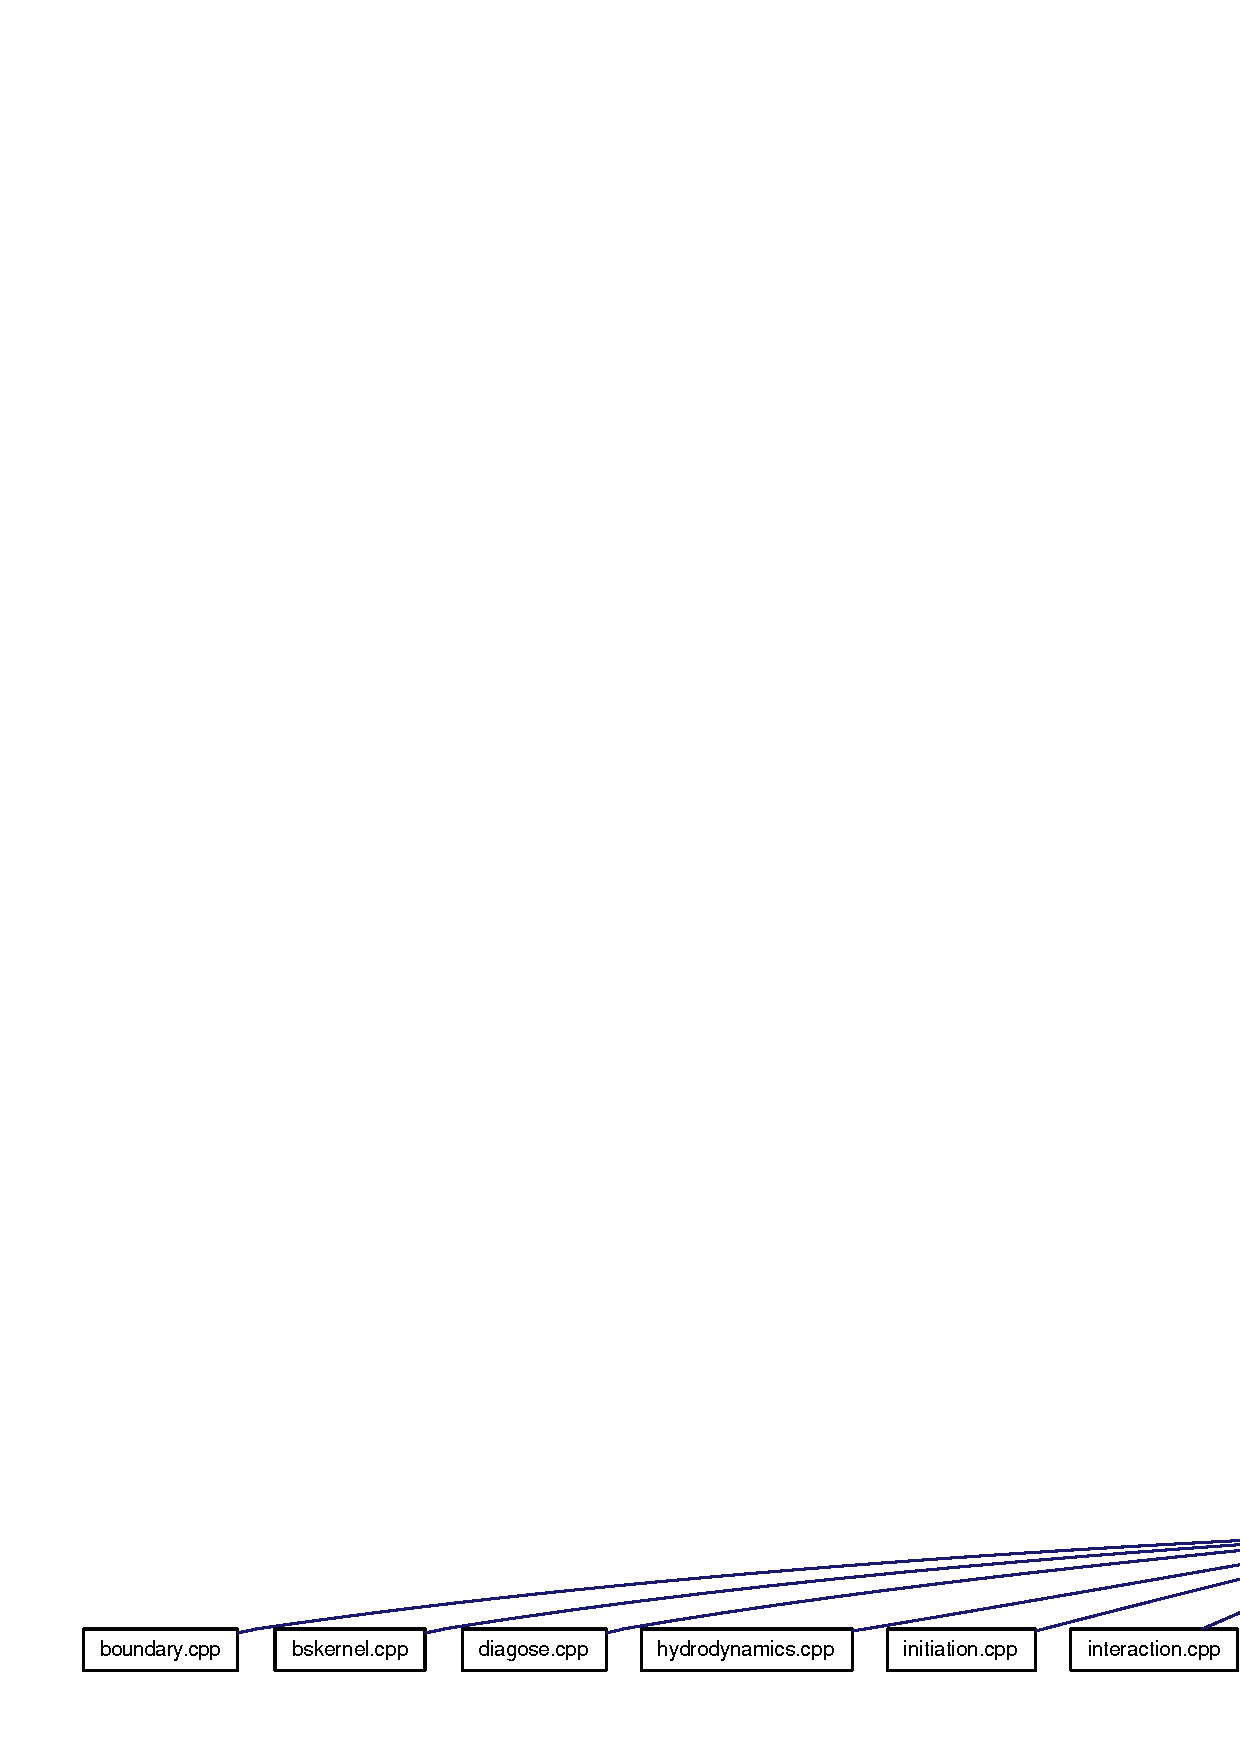
\includegraphics[width=420pt]{timesolver_8h__dep__incl}
\end{center}
\end{figure}
\subsection*{Classes}
\begin{CompactItemize}
\item 
class \hyperlink{classTimeSolver}{TimeSolver}
\begin{CompactList}\small\item\em Time solver class. \item\end{CompactList}\end{CompactItemize}


\label{_details}
\hypertarget{_details}{}
\subsection{Detailed Description}
Time solver class. 

provides methods that iterate over one output time interval (D\_\-time) either with the summation density approach or with the continuity density approach 